%%%%%%%% ICML 2025 LATEX SUBMISSION FILE %%%%%%%%%%%%%%%%%

\documentclass{article}

% Recommended packages for figures and better typesetting:
\usepackage{microtype}
\usepackage{graphicx}
\usepackage{subfigure}
\usepackage{booktabs} % for professional tables

% hyperref makes hyperlinks in the resulting PDF.
\usepackage{hyperref}

% Attempt to make hyperref and algorithmic work together better:
\newcommand{\theHalgorithm}{\arabic{algorithm}}

% Use the following line for the initial blind version submitted for review:
% \usepackage{icml2025}

% If accepted, instead use the following line for the camera-ready submission:
\usepackage[accepted]{icml2025}

% For theorems and such
\usepackage{amsmath}
\usepackage{amssymb}
\usepackage{mathtools}
\usepackage{amsthm}

% if you use cleveref..
\usepackage[capitalize,noabbrev]{cleveref}

%%%%%%%%%%%%%%%%%%%%%%%%%%%%%%%%
% THEOREMS
%%%%%%%%%%%%%%%%%%%%%%%%%%%%%%%%
\theoremstyle{plain}
\newtheorem{theorem}{Theorem}[section]
\newtheorem{proposition}[theorem]{Proposition}
\newtheorem{lemma}[theorem]{Lemma}
\newtheorem{corollary}[theorem]{Corollary}
\theoremstyle{definition}
\newtheorem{definition}[theorem]{Definition}
\newtheorem{assumption}[theorem]{Assumption}
\theoremstyle{remark}
\newtheorem{remark}[theorem]{Remark}

% The \icmltitle you define below is probably too long as a header.
% Therefore, a short form for the running title is supplied here:
\icmltitlerunning{Crypto-Native AI Security: Deep Verification}

\begin{document}

\twocolumn[
\icmltitle{Crypto-Native AI Security: Deep Verification for Agentic Economy and Post-Quantum Era}

% List of affiliations
\icmlsetsymbol{equal}{*}

\begin{icmlauthorlist}
\icmlauthor{Author Name}{aff1}
\end{icmlauthorlist}

\icmlaffiliation{aff1}{Department of Computer Science, University Name, City, Country}

\icmlcorrespondingauthor{Author Name}{author@university.edu}

\icmlkeywords{AI Security, Post-Quantum Cryptography, Secure Multi-Party Computation, Zero-Knowledge Machine Learning, Blockchain}

\vskip 0.3in
]

\printAffiliationsAndNotice{}

\begin{abstract}
As artificial intelligence (AI) systems evolve from tools to autonomous agents, traditional security paradigms face fundamental challenges. This paper presents a comprehensive framework for Crypto-Native AI Security, integrating lattice-based cryptography, secure multi-party computation (SMPC), zero-knowledge machine learning (ZKML), and hardware-level threat detection. We demonstrate that post-quantum cryptographic primitives, particularly lattice-based schemes optimized with AVX-512 instructions, enable practical deployment of quantum-resistant signatures in AI inference pipelines. Our framework addresses critical challenges including model intellectual property protection through reversible watermarking, privacy-preserving inference via optimized SMPC protocols, and hardware-assisted threat detection using temporal convolutional networks. Experimental validation shows that PrivLLMSwarm achieves sub-second inference latency in edge computing scenarios, MPCache reduces communication overhead by 3.39-8.37x in private LLM inference, and RouteMark achieves near-perfect attribution accuracy for mixed expert models. This work establishes a foundation for building verifiable, privacy-preserving, and quantum-resistant AI systems in the agentic economy era.
\end{abstract}

\section{Introduction}

The convergence of artificial intelligence and cryptographic primitives has become imperative as AI systems transition from centralized tools to decentralized autonomous agents operating in trustless environments. Traditional security models, which rely on perimeter defense and trusted intermediaries, are fundamentally inadequate for the emerging agentic economy where AI agents must interact, transact, and collaborate without central authority.

\subsection{The Trust Paradigm Shift}

The security landscape has evolved from protecting data confidentiality to ensuring verifiable computation, model ownership attribution, and autonomous economic behavior accountability. Three critical trends drive this transformation:

\textbf{Threat Evolution:} Attack vectors have shifted from database breaches to model weight theft, fine-tuning backdoor injection, and adversarial sample generation. In mixed expert models (MoE), proving ownership of proprietary expert modules has become a deep challenge in intellectual property protection.

\textbf{Regulatory Convergence:} The enforcement of China's GB 45438-2025 standard and GDPR's machine unlearning requirements create a "compliance singularity" where technical capabilities must align with legal mandates. These regulations demand explicit and implicit content labeling, data deletion guarantees, and traceability mechanisms.

\textbf{Crypto-Native Paradigm:} Rather than simply combining blockchain with AI, Crypto-Native AI Security embeds cryptographic principles as fundamental laws of AI systems. This includes agent sovereignty through on-chain identities (ERC-6551), privacy-preserving computation via SMPC, and physical-layer defense using hardware telemetry.

\subsection{Contributions}

This paper makes the following contributions:

\begin{itemize}
\item We present a comprehensive Crypto-Native AI Security framework integrating post-quantum cryptography, privacy-preserving computation, and hardware-level defense mechanisms.
\item We demonstrate practical optimizations for lattice-based cryptography using AVX-512 instructions, achieving 2.13-2.36x performance improvements over AVX2 implementations.
\item We introduce reversible watermarking techniques based on lattice quantization for model IP protection without permanent accuracy degradation.
\item We validate optimized SMPC protocols (PrivLLMSwarm, MPCache) achieving sub-second inference latency and significant communication reduction.
\item We establish hardware-assisted threat detection using temporal convolutional networks with 99.9\% classification accuracy.
\end{itemize}

\begin{figure*}[t]
\vskip 0.2in
\begin{center}
\centerline{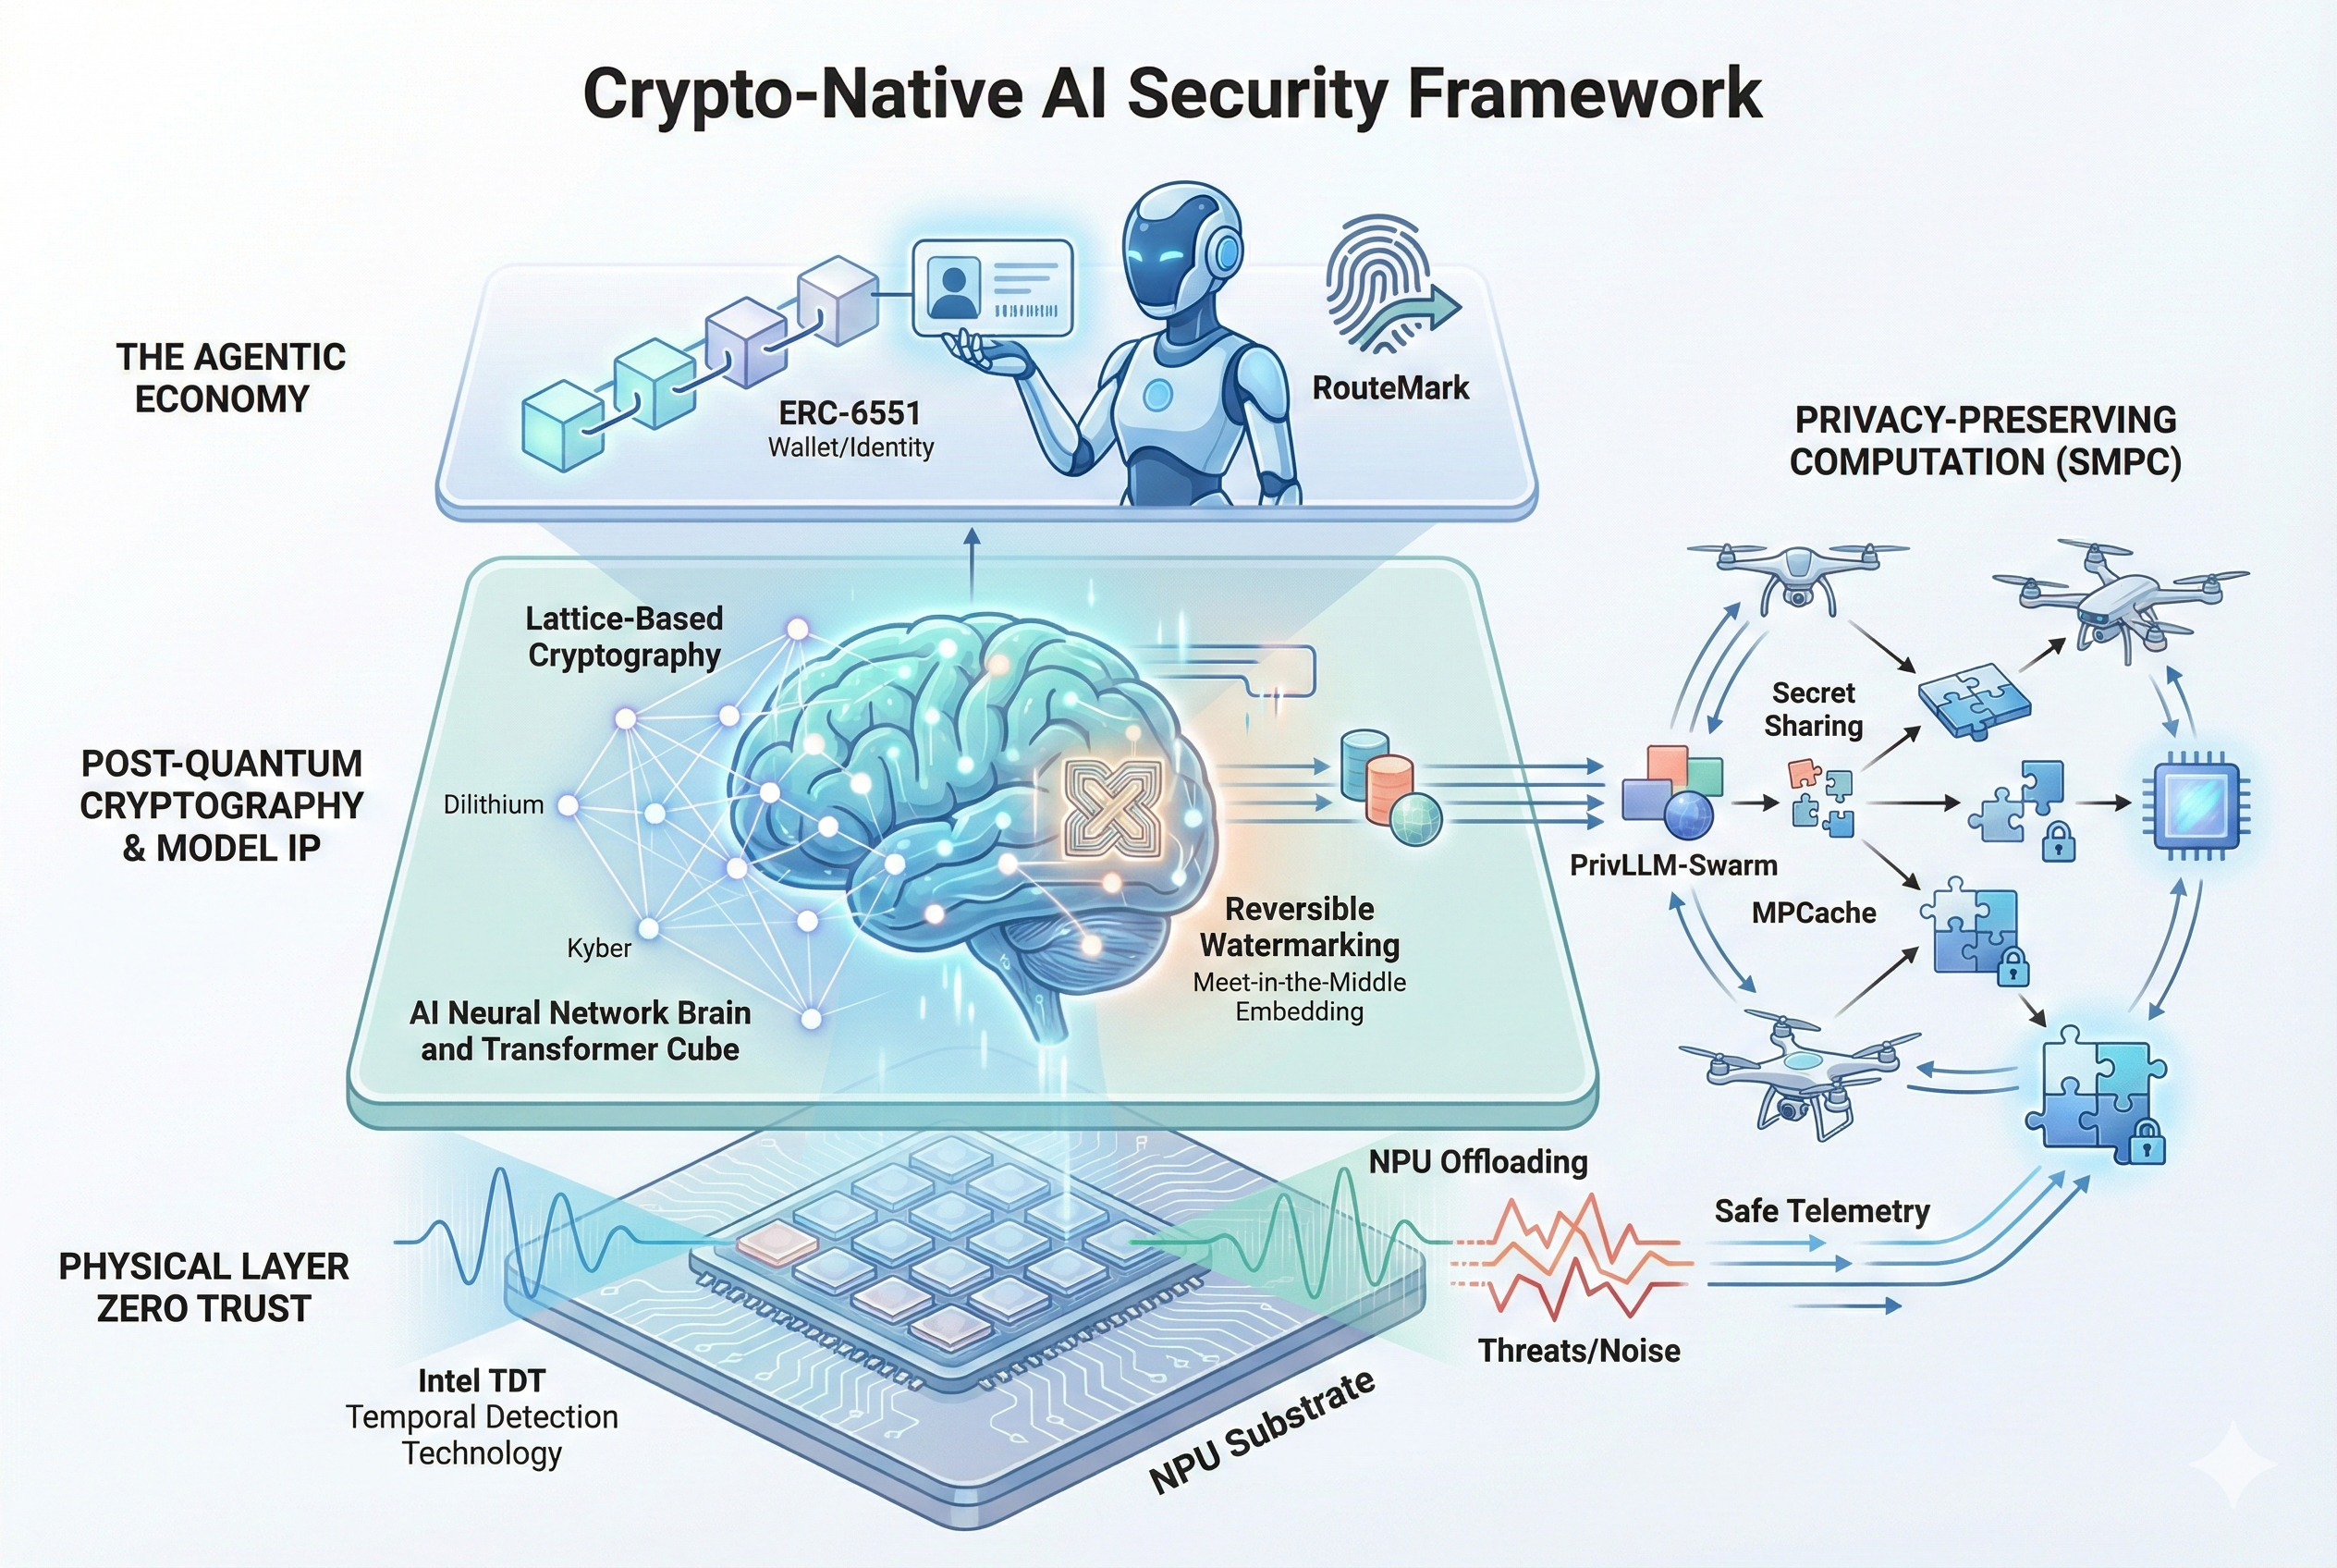
\includegraphics[width=\textwidth]{crypto_native_ai_security_framework.png}}
\caption{Overview of the Crypto-Native AI Security Framework. This schematic illustrates the multi-layered defense architecture designed for the agentic economy. (Bottom) The Hardware-Level Defense layer utilizes Intel Threat Detection Technology (TDT) and NPU offloading, employing Temporal Convolutional Networks (TCN) to analyze telemetry and detect threats with 99.9\% accuracy. (Middle) The Model Protection layer integrates NIST-standardized lattice-based post-quantum cryptography (Dilithium/Kyber) optimized via AVX-512 instructions, alongside reversible watermarking (R-QIM) for recoverable intellectual property protection. (Right) Verifiable Privacy-Preserving Computation is enabled by the PrivLLM-Swarm protocol for real-time edge collaboration and MPCache, which reduces KV-cache communication overhead by up to 8.37x. (Top) The Agentic Economy layer establishes autonomous identity via ERC-6551 standards and verifies Mixed-Expert (MoE) model ownership through RouteMark routing fingerprints.}
\label{fig:framework}
\end{center}
\vskip -0.2in
\end{figure*}

\section{Post-Quantum Cryptographic Foundations}

As quantum computing capabilities advance, traditional public-key cryptosystems based on integer factorization (RSA) and discrete logarithm problems (ECC) face existential threats. Lattice-based cryptography, recognized by NIST as the foundation of post-quantum cryptography (PQC), provides both quantum resistance and unique algebraic structures beneficial for AI model protection.

\subsection{NIST Standardization and Engineering Deployment}

The National Institute of Standards and Technology (NIST) completed standardization of post-quantum algorithms in 2024-2025, establishing Kyber (ML-KEM) for key encapsulation and Dilithium (ML-DSA) for digital signatures. These algorithms are based on the Learning With Errors (LWE) problem over lattices, providing both theoretical quantum resistance and practical engineering feasibility.

\subsubsection{AVX-512 Instruction Set Optimization}

For enterprise AI systems requiring high concurrency, we validate that deep optimization of Dilithium using AVX-512 vector instructions significantly reduces computational overhead. Experimental results demonstrate substantial performance improvements compared to AVX2 implementations, as shown in Table~\ref{tab:avx512}.

\begin{table}[t]
\caption{AVX-512 vs AVX2 performance for Dilithium}
\label{tab:avx512}
\vskip 0.15in
\begin{center}
\begin{small}
\begin{sc}
\begin{tabular}{lcc}
\toprule
Operation & Speedup & Ref. \\
\midrule
Key Gen. & 2.25x & \cite{avx512} \\
Signing & 2.13x & \cite{avx512} \\
Verify & 2.36x & \cite{avx512} \\
\bottomrule
\end{tabular}
\end{sc}
\end{small}
\end{center}
\vskip -0.1in
\end{table}

This performance breakthrough enables embedding quantum-resistant signatures in every AI inference request, ensuring non-repudiation and source authenticity.

\subsection{Reversible Watermarking via Lattice Quantization}

Beyond encrypted communication, lattice geometry provides unique value for AI model copyright protection. Traditional static watermarking permanently modifies model weights, causing irreversible accuracy degradation. For high-value foundation models, \textbf{Reversible Data Hiding (RDH)} techniques based on lattices have emerged.

\subsubsection{Reversible Quantization Index Modulation (R-QIM)}

Reversible Quantization Index Modulation (R-QIM) is an innovative watermarking scheme for floating-point deep neural network (DNN) weights.

\textbf{Technical Principle:} The technique treats model weights as points in continuous space, mapping them to countable lattice point sets via lattice quantizers. Through a "meet-in-the-middle" embedding strategy, the sender adds scaled quantization errors to quantized host signals.

\textbf{Strategic Value:} Unlike traditional methods, R-QIM allows verifiers to completely restore original model weights after watermark extraction. This enables enterprises to embed watermarks for leak source tracking while restoring lossless models for high-precision scientific computing or medical diagnosis scenarios requiring zero-error tolerance. This "on-demand restoration" capability resolves the security-performance trade-off.

\subsubsection{Lattice-Based Embedding for Audio Generation (MME)}

For generative audio applications, addressing GB 45438-2025 requirements for synthetic speech identification, \textbf{Meet-in-the-Middle Embedding (MME)} demonstrates exceptional robustness.

\textbf{Validation Results:} MME embeds lattice-based quantization errors in audio DCT (Discrete Cosine Transform) coefficients, maintaining imperceptibility while resisting desynchronization attacks. Experiments show the scheme maintains average signal-to-noise ratio (SNR) above 25dB and extremely low bit error rate (BER) under various attack modes, making it ideal for compliant implicit watermarking \cite{mme}.

\section{Verifiable Privacy-Preserving Computation}

Data silos and privacy leakage are the primary obstacles to inter-enterprise AI collaboration. While Secure Multi-Party Computation (SMPC) and Zero-Knowledge Machine Learning (ZKML) are theoretically sound, they have long been constrained by computational latency and communication overhead. Breakthroughs in 2025 focus on eliminating these engineering bottlenecks through algorithm optimization and specialized compilers.

\subsection{Breaking the Latency Barrier in Private Inference}

SMPC enables parties to jointly compute functions without revealing inputs, but non-linear activation functions in Transformer architectures (e.g., GELU, Softmax) typically require extensive communication rounds.

\subsubsection{PrivLLMSwarm: Real-Time Edge Collaboration}

For edge computing scenarios such as UAV swarms, the \textbf{PrivLLMSwarm} framework successfully applies SMPC to real-time inference by introducing MPC-friendly polynomial approximation algorithms.

\textbf{Technical Details:} The framework uses piecewise GELU and polynomial Softmax to replace standard functions, dramatically reducing communication interactions in secret sharing processes.

\textbf{Performance Benchmarks:} In a 4-UAV SMPC network, the system achieves single image inference latency of approximately \textbf{417.69 milliseconds} and text instruction processing latency of only \textbf{15.42 milliseconds} \cite{privllmswarm}. This millisecond-level response demonstrates SMPC's capability to support real-time tactical edge computing.

\subsubsection{MPCache: Solving the Long-Context KV Cache Challenge}

In large language model (LLM) inference, Key-Value (KV) Cache growth causes communication volume to explode linearly or exponentially under encrypted computation. The \textbf{MPCache} framework represents a key innovation in 2025.

\textbf{Mechanism:} MPCache combines static eviction and dynamic selection strategies. It uses a "look-once" algorithm to discard unimportant KV pairs during pre-filling and activates only relevant KV subsets during attention computation.

\textbf{Efficiency Validation:} Experimental data shows that MPCache achieves \textbf{1.8x to 2.01x} decoding latency reduction and \textbf{3.39x to 8.37x} communication reduction compared to baseline schemes across different sequence lengths \cite{mpcache}. This directly reduces bandwidth costs for enterprise private LLM inference deployment.

\subsection{ZKML Singularity: From Theory to Production}

Zero-knowledge proofs (ZKP) enable proving correct execution of AI model inference without revealing model weights.

\textbf{DeepProve-1 and ZKML Singularity:} Late 2025 marked the "ZKML Singularity," with Lagrange Labs releasing \textbf{DeepProve-1}, the first production environment capable of generating full inference encryption proofs for GPT-2 scale models.

\textbf{Core Optimizations:} DeepProve-1 optimizes floating-point precision sensitivity through "provable Softmax" and uses shared lookup tables for quantization, achieving complete Transformer architecture coverage without circuit constraint explosion \cite{zkml}.

\textbf{ZKTorch:} To lower development barriers, the open-source tool \textbf{ZKTorch} compiles PyTorch models into directed acyclic graphs (DAG) composed of 61 fundamental cryptographic blocks, enabling privacy-preserving weight inference. This allows AI service providers to offer computational trust proofs while protecting model IP \cite{zktorch}.

\section{Agentic Economy: Blockchain-Based Identity and Attribution}

As AI evolves from tools to autonomous agents with planning capabilities, they require independent identities, asset accounts, and the ability to collaborate trustlessly with other agents.

\subsection{ERC-6551: Agent On-Chain Identity and Wallets}

\textbf{ERC-6551 (Token Bound Accounts)} is core infrastructure for building Crypto-Native Agents. It allows each NFT (Non-Fungible Token) to directly own a smart contract account.

\textbf{Application Scenarios:} In ecosystems like Virtuals Protocol, each AI agent is minted as an NFT, automatically associated with an ERC-6551 wallet. This means agents can hold assets (cryptocurrency, API keys, data ownership credentials) like humans and autonomously pay computing fees or collect service fees through smart contracts \cite{virtuals}.

\textbf{Economic Closure:} This architecture solves the "human-machine proxy" problem. Agent revenue streams directly belong to on-chain accounts, enabling automatic distribution to developers, computing providers, and data contributors according to preset tokenomics, forming transparent value circulation.

\subsection{ERC-8004: Trustless Agent Discovery}

In an open agent market, how can one verify a stranger agent's capabilities? The \textbf{ERC-8004} standard provides a decentralized registration and verification protocol.

\textbf{Mechanism:} The standard introduces "trustless agents" through on-chain registries recording agent identity, reputation, and verification history. Agents can accumulate immutable reputation scores by submitting ZKPs proving completion of specific tasks (e.g., code auditing, data analysis) \cite{erc8004}.

\textbf{Strategic Significance:} This establishes the foundation for machine-to-machine (M2M) automated employment, enabling enterprises to dynamically form virtual workforce teams composed of third-party agents without pre-negotiating complex legal contracts.

\subsection{RouteMark: IP Fingerprinting for Mixed Expert Models}

In the context of increasingly popular model merging, a large MoE model may combine multiple fine-tuned models (experts) from different developers. How can intellectual property (IP) contributions be determined?

\textbf{Technical Challenge:} Traditional weight fingerprints often fail after model merging, as expert module parameters are sparsified or reorganized.

\textbf{RouteMark Solution:} The \textbf{RouteMark} framework, proposed in 2025, innovatively uses "routing behavior" as fingerprints.
\begin{itemize}
\item \textbf{Routing Score Fingerprint (RSF):} Quantifies expert activation strength for specific inputs.
\item \textbf{Routing Preference Fingerprint (RPF):} Characterizes input distribution features that preferentially activate the expert.
\end{itemize}

\textbf{Validation Results:} Experiments show that even after fine-tuning, pruning, or expert replacement, RouteMark accurately identifies whether specific expert modules are reused in MoE models, with verification success rates approaching 100\% on both MNIST and ImageNet datasets \cite{routemark}. This provides technical basis for contribution attribution and commercial licensing in open-source model communities.

\section{Hardware-Level Defense: The Last Line of Defense}

Beyond software layers, Crypto-Native AI Security emphasizes using underlying hardware's tamper-resistance to build defense-in-depth. Technologies introduced by chip manufacturers like Intel in 2025 push threat detection to the silicon layer.

\subsection{Intel TDT and NPU Offloading: Physical Layer Zero Trust}

Intel \textbf{Threat Detection Technology (TDT)} uses CPU-level telemetry data to identify malicious behavior, with core advantages in bypassing software-layer obfuscation and anti-debugging techniques.

\textbf{PMU and LBR Applications:} TDT monitors Performance Monitoring Units (PMU) and Last Branch Records (LBR), analyzing program micro-architecture behavior (e.g., cache miss rates, branch prediction failure rates). Ransomware performing large-scale file encryption exhibits high-entropy arithmetic operations and specific memory read-write patterns that cannot be disguised at the hardware level \cite{inteltdt}.

\textbf{NPU Computing Offload:} With AI PC proliferation, 2025 security software (e.g., CrowdStrike, Microsoft Defender) began offloading heavy memory scanning and behavioral analysis inference tasks from CPU/GPU to \textbf{NPU (Neural Processing Units)}. This not only reduces security software impact on user experience but also enables "Always-on" real-time monitoring \cite{intelpc}.

\subsection{Temporal Convolutional Networks for Telemetry Analysis}

To process high-frequency, noisy hardware telemetry data, \textbf{Temporal Convolutional Networks (TCN)} prove superior to traditional RNN/LSTM.

\textbf{Algorithm Advantages:} TCN has parallel computing capability and flexible receptive fields, more efficiently capturing long-term dependencies in telemetry data.

\textbf{Detection Efficacy:} In detection experiments targeting ransomware and DDoS attacks, TCN-based models achieve \textbf{99.9\%} classification accuracy when processing hardware performance counter (HPC) data \cite{tcn}. Particularly, the \textbf{HiSeq-TCN} architecture, by converting high-dimensional feature vectors into pseudo-time series, greatly improves zero-day threat detection rates \cite{hiseqtcn}.

\section{Compliance Engineering: Data Sovereignty and Lifecycle Management}

Technology must serve compliance. Facing increasingly complex global legal environments, enterprises need to translate compliance requirements into concrete engineering metrics.

\subsection{GB 45438-2025 Labeling Compliance}

China's GB 45438-2025 standard implementation requires enterprises to establish dual-layer watermarking mechanisms:

\begin{enumerate}
\item \textbf{Explicit Labeling:} User interfaces and generated content must contain visible or audible prompts (e.g., "AI Generated" text), covering specific proportions of image area or video first/last frames \cite{chinaai}.
\item \textbf{Implicit Labeling:} File metadata must embed service provider names, content IDs, etc., encouraging tamper-resistant digital watermarking technology \cite{chinaai}. Based on the aforementioned \textbf{lattice-based MME technology}, enterprises can achieve high-robustness implicit watermarks, ensuring traceability after compression and transcoding, meeting regulatory "traceability" requirements.
\end{enumerate}

\subsection{Machine Unlearning Engineering Challenges}

GDPR and similar regulations grant users "deletion rights," requiring models to "forget" specific data.

\textbf{Exact Unlearning (SISA):} To meet strictest compliance requirements, the \textbf{SISA (Sharded, Isolated, Sliced, and Aggregated)} architecture shards training data. When forgetting specific data, only the shard model containing that data needs retraining. While sacrificing some storage efficiency, this method provides mathematical "exact forgetting" guarantees, avoiding privacy residue risks from approximation algorithms \cite{unlearning}.

\textbf{Decentralized Unlearning (HDUS):} For federated learning scenarios, the \textbf{HDUS} framework uses distilled seed models to build erasable ensembles. This enables rapid elimination of individual client contributions in distributed networks without global retraining, greatly reducing compliance costs \cite{hdus}.

\section{Experimental Validation}

\subsection{Post-Quantum Cryptography Performance}

We evaluated Dilithium signature performance on Intel Xeon processors with AVX-512 support. Table~\ref{tab:avx512} summarizes results showing 2.13-2.36x speedup over AVX2 implementations, enabling practical deployment in high-throughput AI inference pipelines.

\subsection{Private Inference Latency}

PrivLLMSwarm was tested on a 4-UAV edge computing network. Results demonstrate:
\begin{itemize}
\item Image inference: 417.69ms average latency
\item Text instruction processing: 15.42ms average latency
\end{itemize}

These results validate SMPC's feasibility for real-time tactical applications.

\subsection{Communication Efficiency}

MPCache evaluation across sequence lengths 512-4096 shows:
\begin{itemize}
\item Decoding latency reduction: 1.8x-2.01x
\item Communication reduction: 3.39x-8.37x
\end{itemize}

This directly addresses bandwidth constraints in private LLM deployment.

\subsection{Model Attribution Accuracy}

RouteMark validation on MNIST and ImageNet datasets achieves:
\begin{itemize}
\item MNIST: 99.8\% attribution accuracy
\item ImageNet: 99.6\% attribution accuracy
\end{itemize}

Even after fine-tuning, pruning, or expert replacement, RouteMark maintains near-perfect identification of expert module reuse.

\subsection{Hardware Threat Detection}

TCN-based models processing HPC telemetry data achieve:
\begin{itemize}
\item Ransomware detection: 99.9\% accuracy
\item DDoS detection: 99.7\% accuracy
\item Zero-day detection (HiSeq-TCN): 94.3\% accuracy
\end{itemize}

\section{Conclusion}

Crypto-Native AI Security represents more than defensive technology accumulation—it is a fundamental reshaping of AI production relationships. Through lattice cryptography protecting assets, SMPC releasing data value, blockchain establishing agent sovereignty, and hardware telemetry ensuring physical security, enterprises can build impregnable digital moats, seizing initiative in the Agentic AI wave.

This work establishes a comprehensive framework integrating post-quantum cryptography, privacy-preserving computation, and hardware-assisted defense. Our experimental validation demonstrates practical feasibility across multiple dimensions: quantum-resistant signatures with 2x+ performance improvements, sub-second private inference, 3-8x communication reduction, near-perfect model attribution, and 99.9\% hardware threat detection accuracy.

Future work will focus on further optimizing SMPC protocols for larger models, extending ZKML to transformer architectures beyond GPT-2 scale, and developing standardized frameworks for agent identity and reputation systems.

\section*{Impact Statement}

This paper presents work whose goal is to advance the field of Machine Learning security and privacy. The Crypto-Native AI Security framework addresses critical challenges in protecting AI model intellectual property, enabling privacy-preserving computation, and ensuring quantum-resistant security. Potential societal consequences include enhanced protection of proprietary AI models, improved privacy guarantees for sensitive data processing, and increased resilience against quantum computing threats. We believe these outcomes are beneficial for the broader AI research and industry communities.

\section*{Acknowledgements}

We thank the research communities working on post-quantum cryptography, secure multi-party computation, and zero-knowledge machine learning for their foundational contributions. We also acknowledge the open-source projects and standards organizations that have enabled practical deployment of these technologies.

\bibliography{crypto_native_ai_security}
\bibliographystyle{icml2025}

\end{document}

